\chapter{Descripción las herramientas implementadas}\label{chapter:implementation}
En este capítulo se presenta la propuesta de solución para 
la informatización de los procesos de asignación de docencia y 
planificación de las tesis que se llevan a cabo 
en la Facultad de Matemática y Computación de la Universidad de La Habana. 

Se implementó un sistema de gestión siguiendo el modelo cliente-servidor. El desarrollo del servidor se efectuó con el uso Django, en 
particular Django Rest Framework y el cliente se desarrolló utilizando
Quasar para la creación de las interfaces de usarios. Para la administración de la 
base de datos se utilizó el SGBD SQLite. Como resultado se creó una 
aplicación web, cuyo funcionamiento se describe a continuación.

FOTO DE LA VISTA HOME 
ALGO COMO AQUI SE DECIDE QUE PROCESOS SE QUIEREN REALIZAR




\section{Asignación de docencia}



El proceso de asignación de docencia en un departamento se realiza en la 
interfaz que se muestra en la figura \ref{img-ta-done}. El usuario de la 
aplicación puede ver la carga docente de los profesores durante el proceso 
de asignación, realizar filtrados por profesor para ver las asignaturas 
que tiene asignada y descargar un documento CSV que contiene la información 
de la docencia una vez haya terminado la asignación.


\begin{figure}[H]
    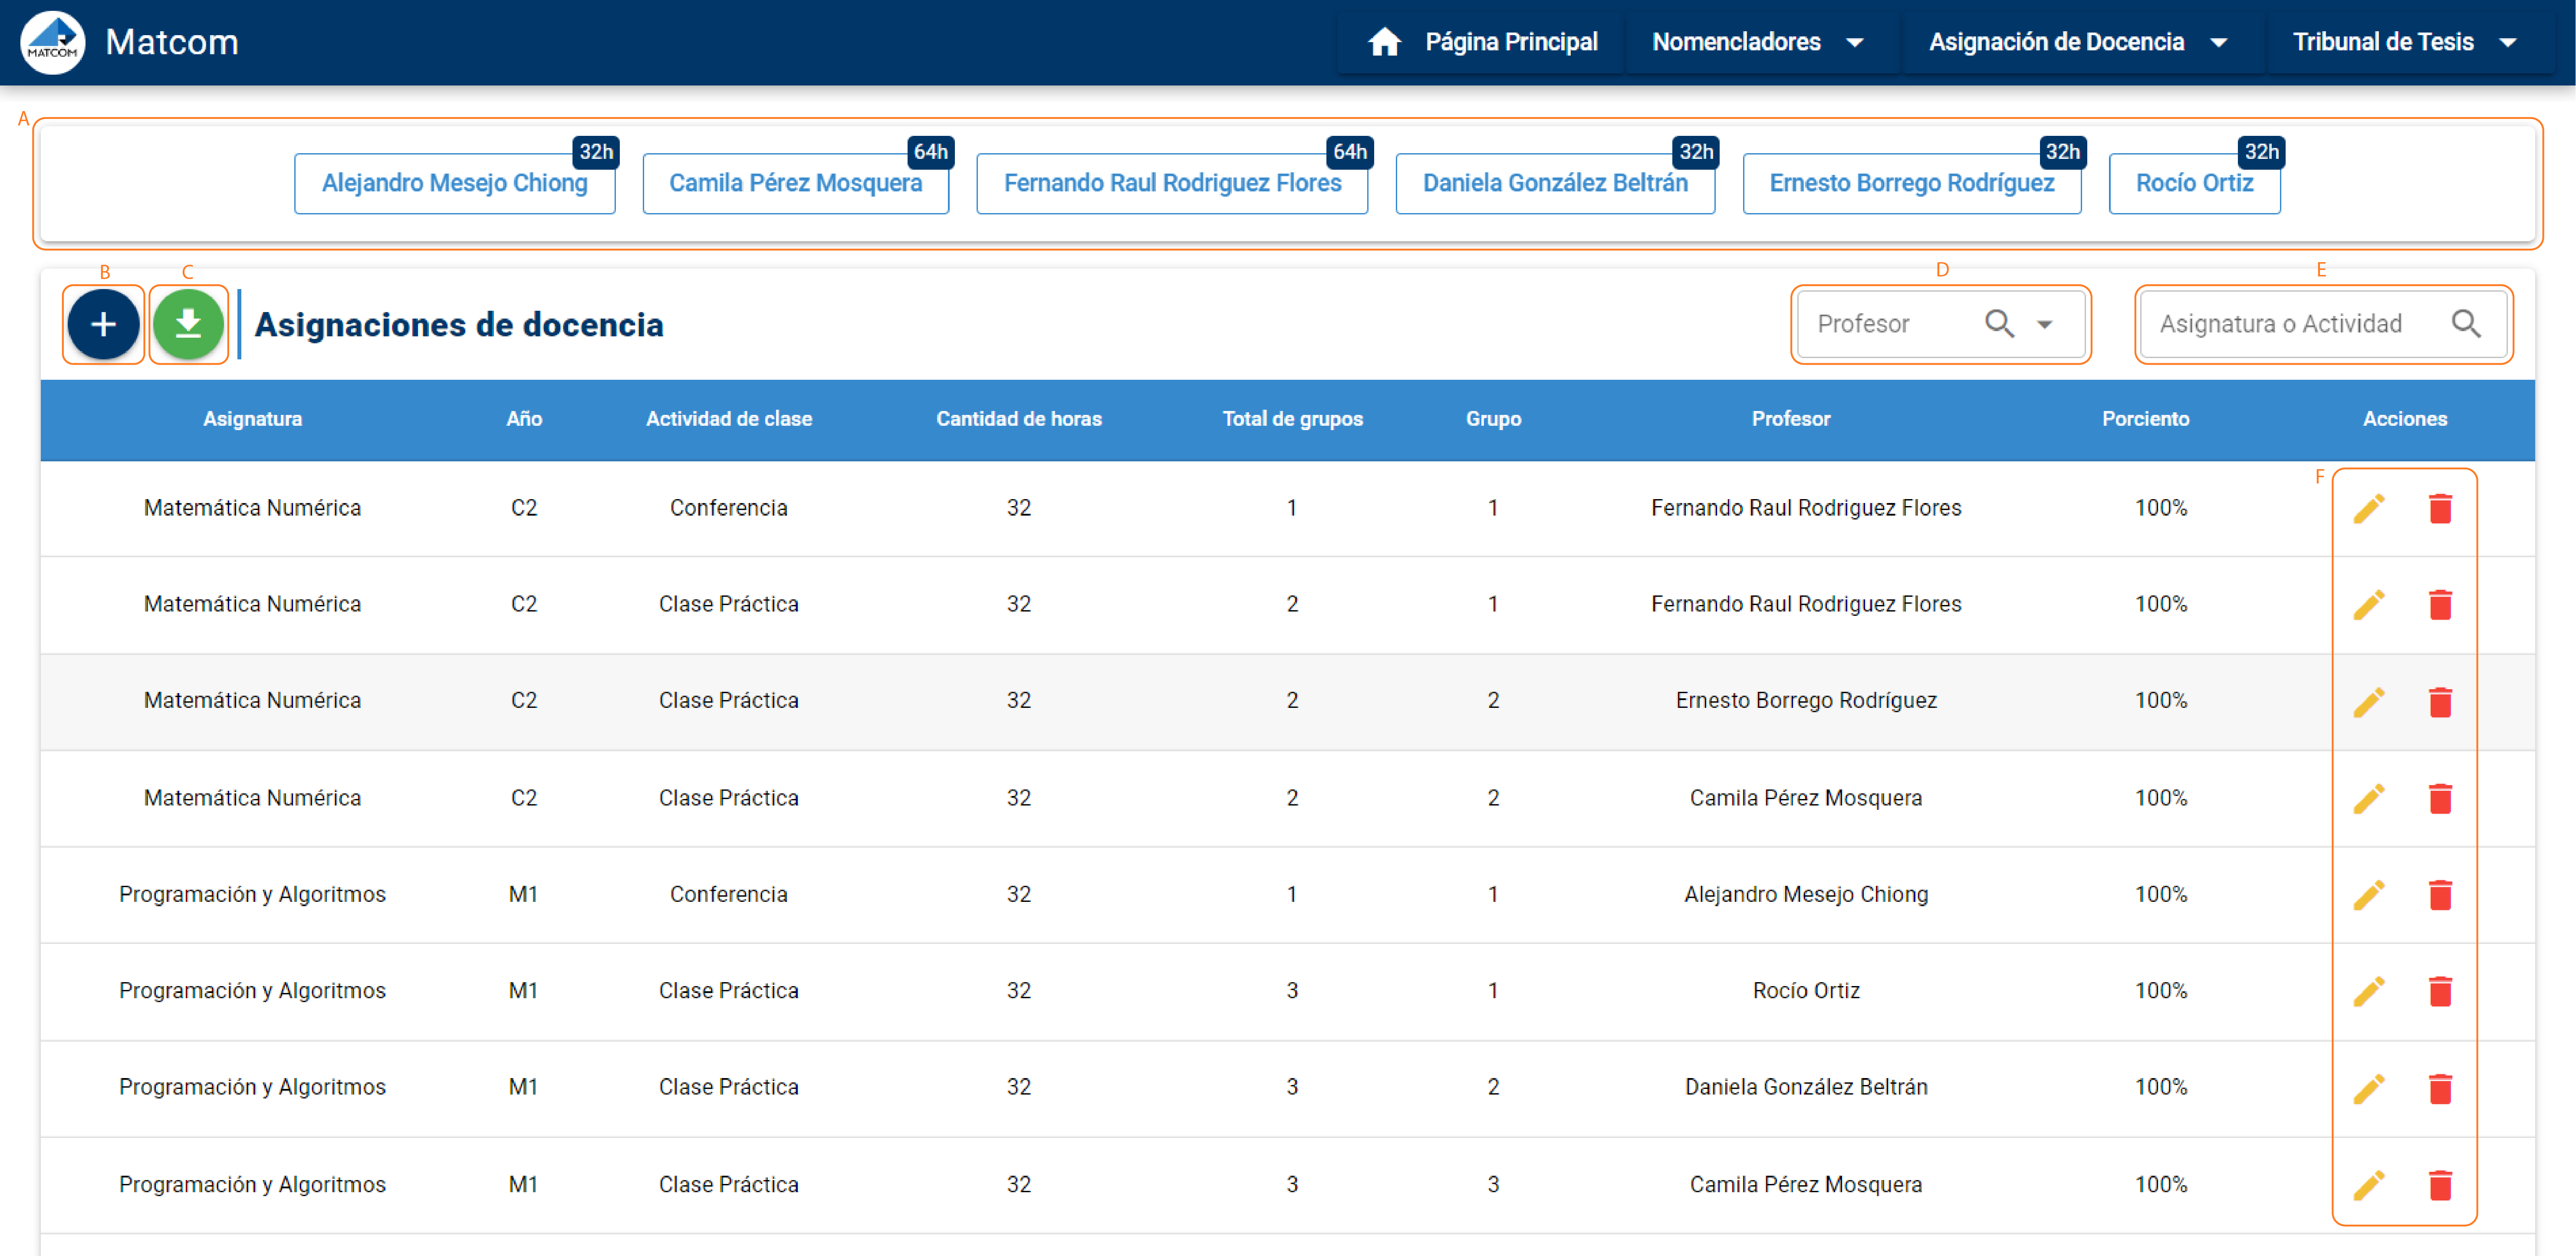
\includegraphics[scale=0.3]{Graphics/Implementation/Docencia/AD-asignada.png}
    \caption{Vista de la asignación de docencia}
    \label{img-ta-done}
\end{figure}

En la figura \ref{img-ta-done},
se indican con recuadros cuatro regiones cuyo significado se explica a continuación.

\begin{itemize}
    \item A: muestra la carga docente de los profesores dada la asignación actual.
    \item B: botón para agregar una nueva planificación de docencia.
    \item C: botón para descargar la asignación de docencia actual.
    \item D: realizar filtrado por los profesores para ver las asignturas que tiene asignadas.
    \item E: realizar búsquedas por las asignaturas o actividades de clase.
    \item F: botones para editar o borrar una fila de la tabla.  
\end{itemize}



En la figura \ref{img-ta-ordering} se muestra como quedaría ordenada la tabla a partir de los profesores,
con el objetivo de mostrar primero aquellas 
asignaturas que no se han asignado aún.


\begin{figure}[H]
    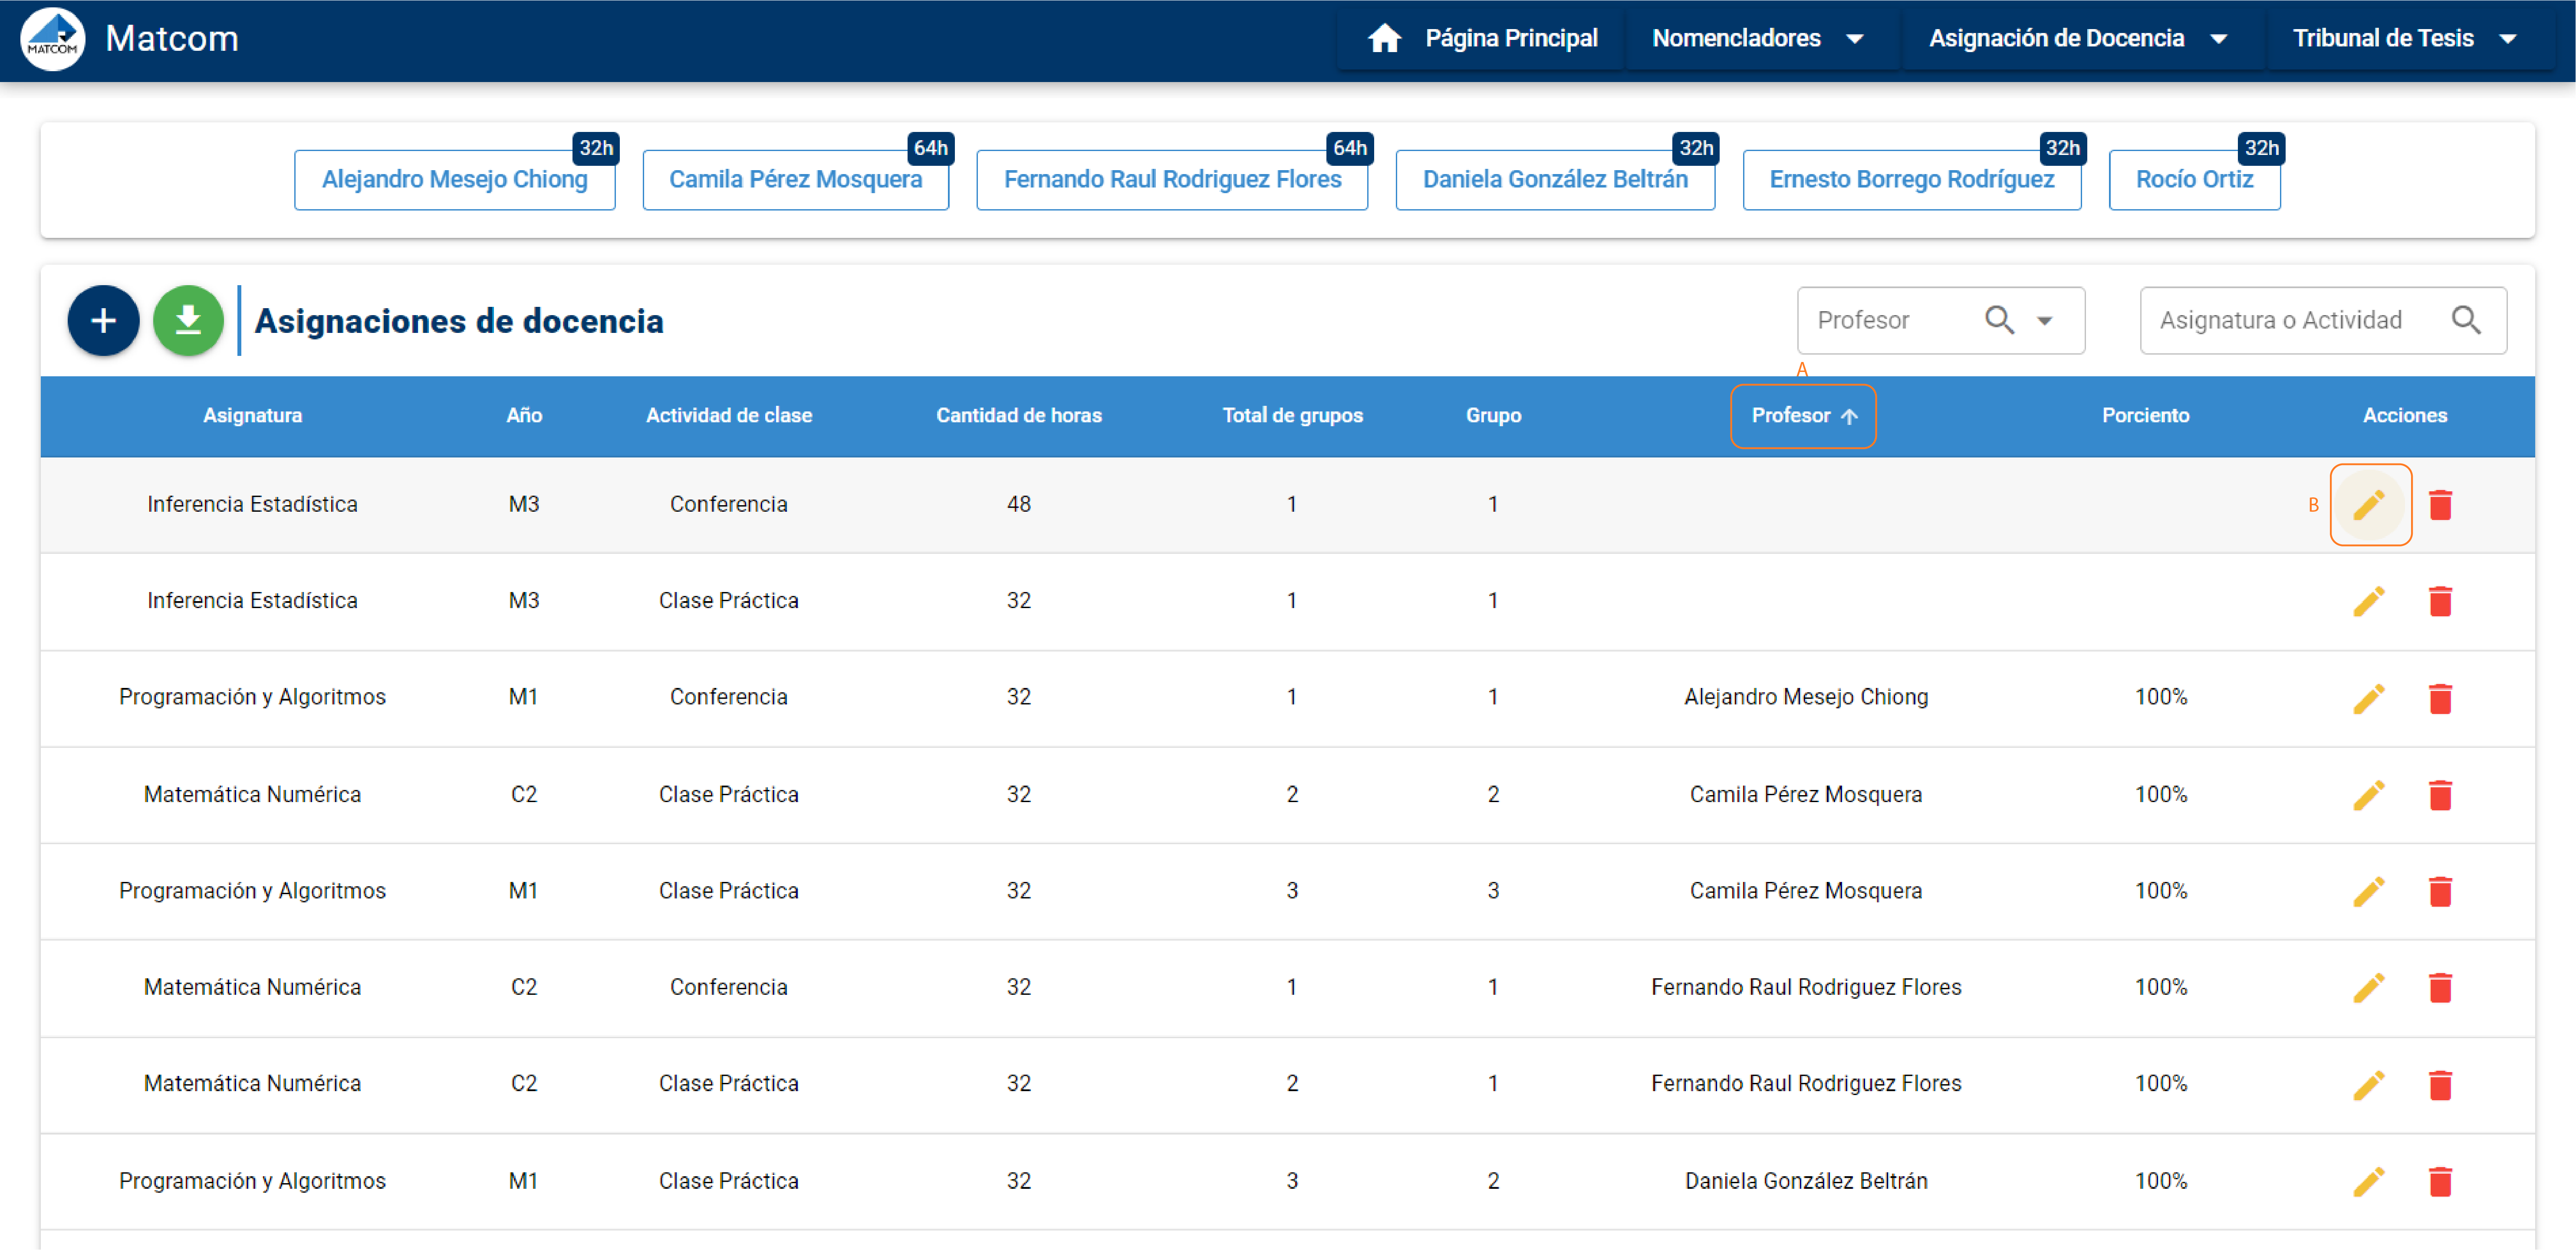
\includegraphics[scale=0.3]{Graphics/Implementation/Docencia/AD-sin-asignar.png}
    \caption{Vista de la asignación de docencia, ordenada por profesores para que aparezcan primero las asignaturas que aún no han sido asignadas}
    \label{img-ta-ordering}
\end{figure}


Para ordenar la tabla a partir de los profesores se debe pulsar sobre el elemento que se indica en 
con el recuadro A. Para realizar una asignación se debe pulsar el botón de editar que se indica con
con el recuadro B. La figura \ref{img-ta-edit-form1} muestra la vista después de pulsar el botón de 
editar.  



\begin{figure}[H]
    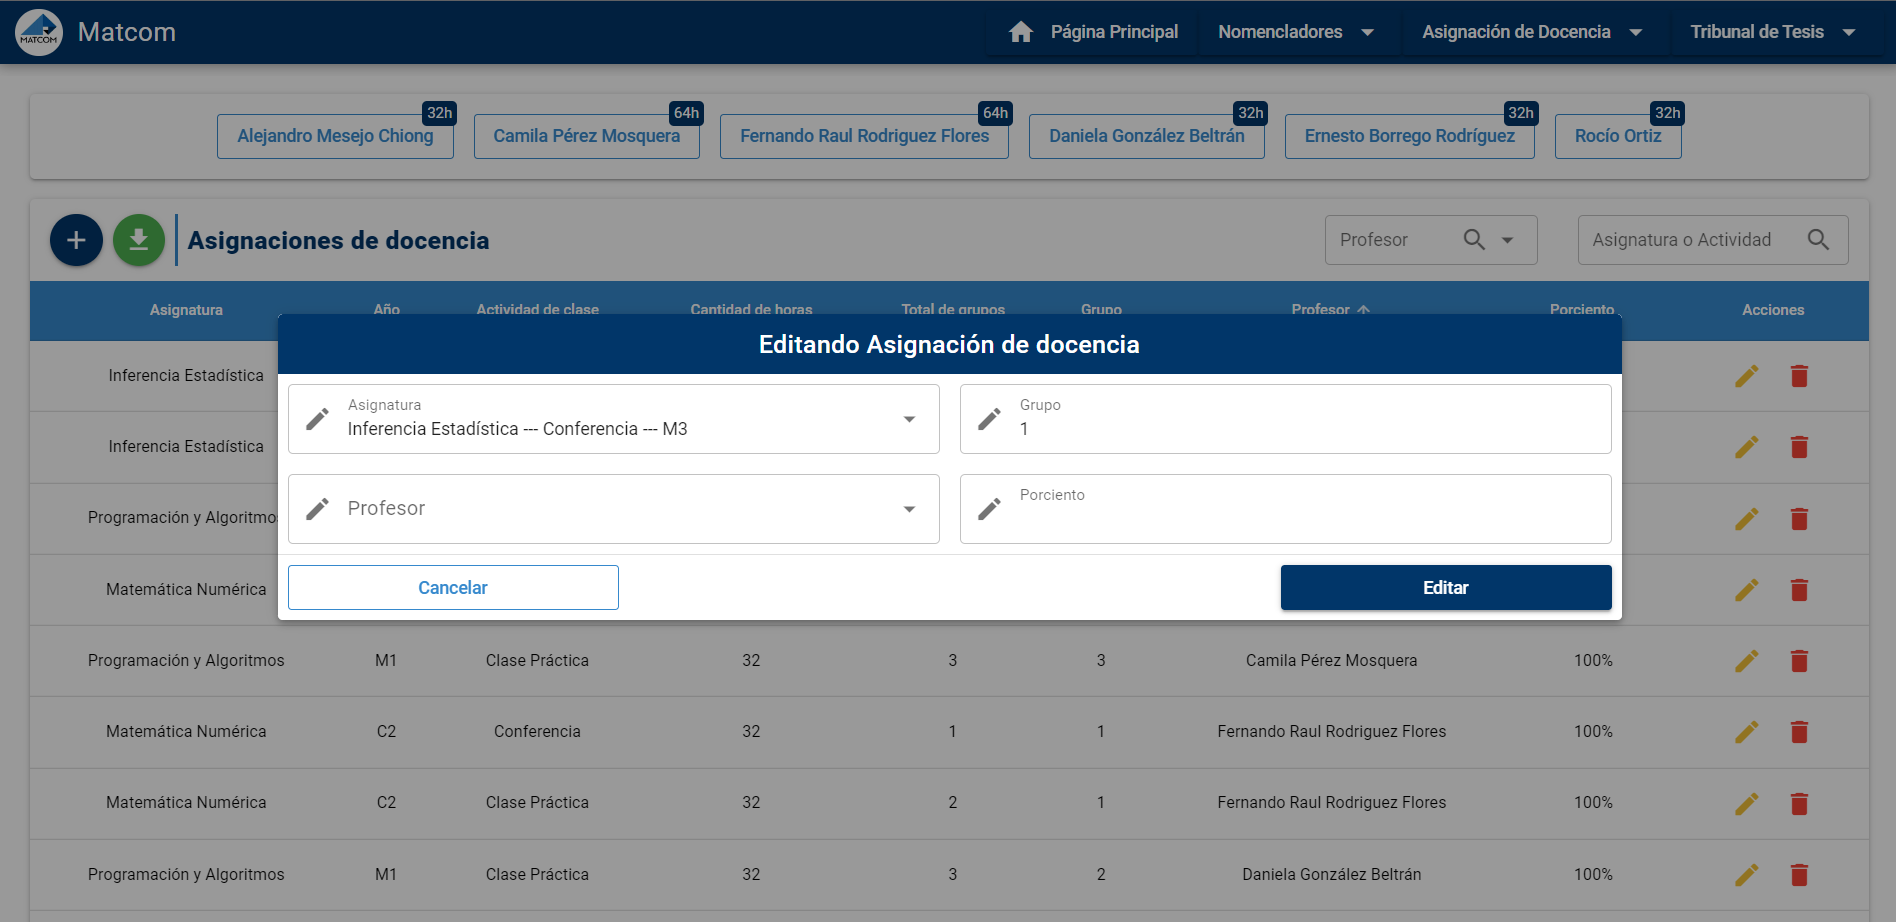
\includegraphics[scale=0.3]{Graphics/Implementation/Docencia/AD-edit-form.png}
    \caption{Vista del formulario para editar una asignación de docencia}
    \label{img-ta-edit-form1}
\end{figure}


Cuando se edita una asignación de docencia es necesario definir la planificación de 
la asignatura (Inferencia Estadística---Conferencia---M3), grupo, profesor que se 
desea asignar y el porciento total de horas que impartirá el profesor. En la figura
\ref{img-ta-edit-form2} se muestra como asignar a la profesora Vivian Sistaschs con un 100
porciento de las horas que se deben impartir en la planificación de la asignatura Inferencia Estadística. 

\begin{figure}[H]
    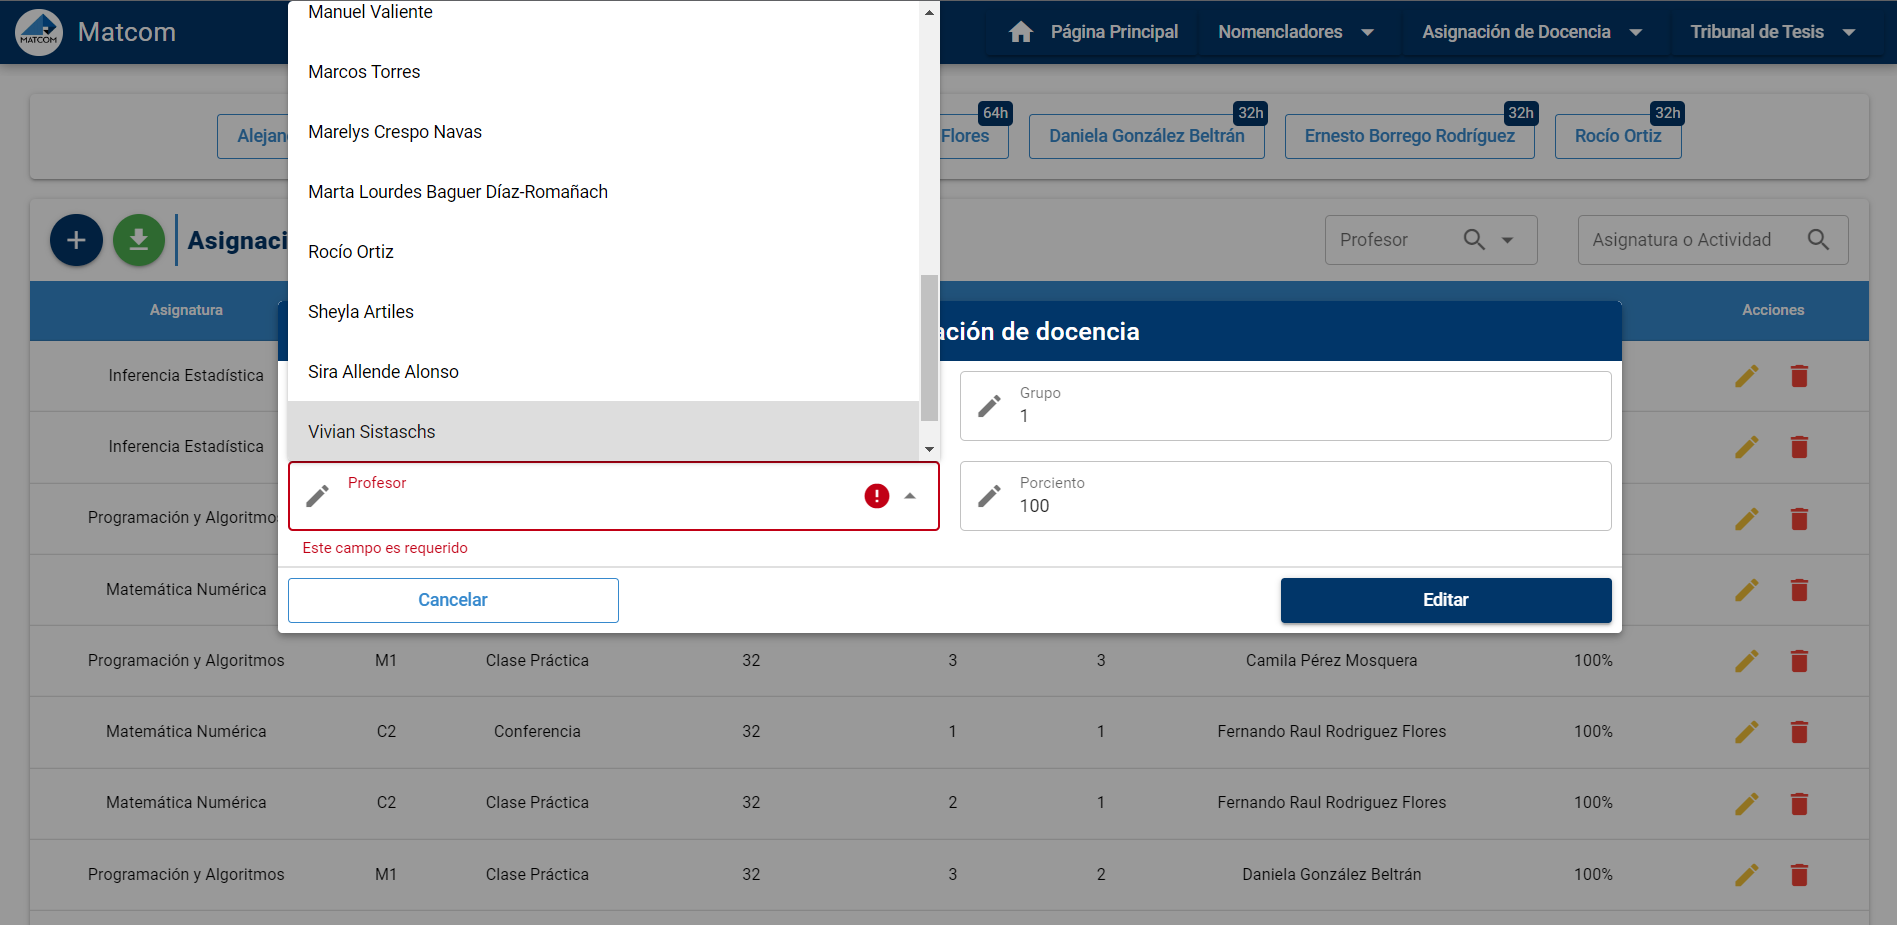
\includegraphics[scale=0.3]{Graphics/Implementation/Docencia/AD-edit-form2.png}
    \caption{Vista del formulario para editar una asignación de docencia, mostrando los profesores posibles para la asignación}
    \label{img-ta-edit-form2}
\end{figure}



La figura \ref{img-ta-result} muestra el resultado de completar los pasos
que se muestran en la figuras \ref{img-ta-ordering}, \ref{img-ta-edit-form1} y \ref{img-ta-edit-form2}.

\begin{figure}[H]
    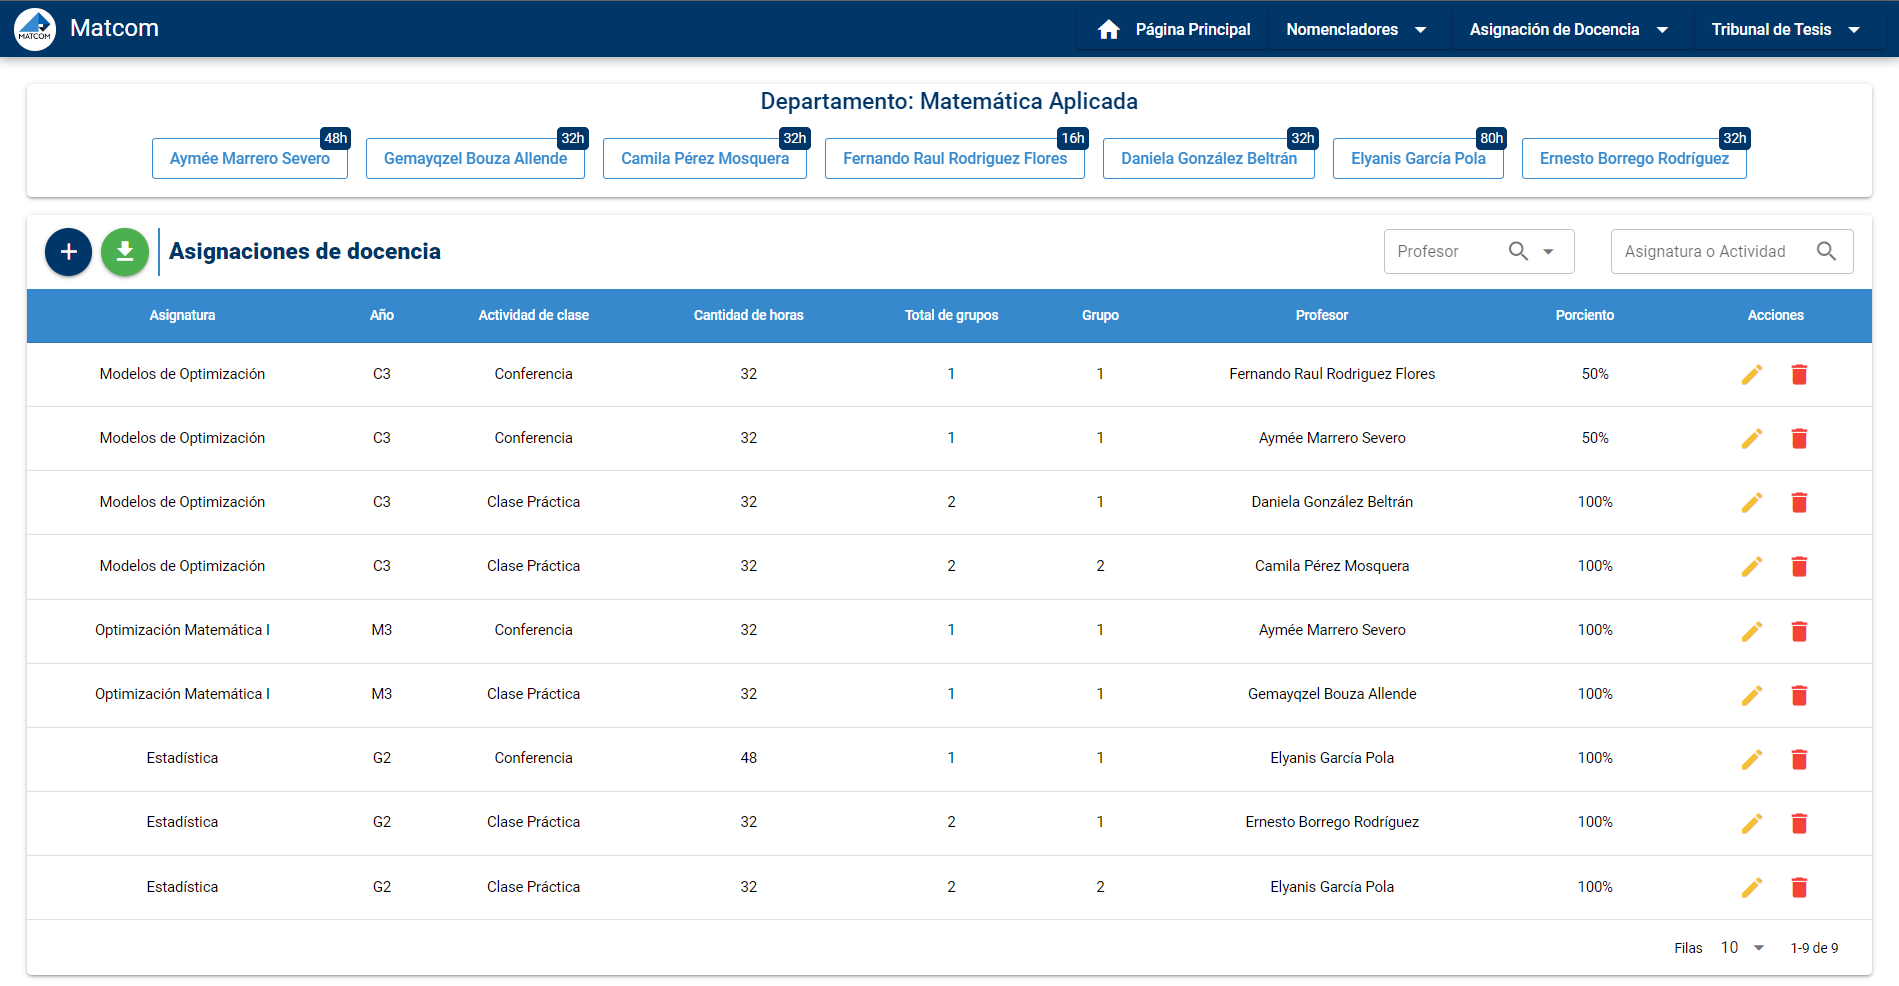
\includegraphics[scale=0.3]{Graphics/Implementation/Docencia/AD-result.png}
    \caption{Vista de la asignación tras realizar una asignación correctamente}
    \label{img-ta-result}
\end{figure}

Cada vez que se realicen cambios en la tabla, ya sean por agregar, editar o eliminar 
asignaciones de docencia, la carga docente de los profesores se actualiza como se indica 
en el recuadro A. El recuadro B refleja como quedó la fila tras la asignación de la profesora 
Vivian Sistaschs para que imparta las 48 horas de conferencia de la asignatura Inferencia Matemática
a los estudiantes que cursan el tercer año de la carrera Matemática.


Para poder llevar a cabo el proceso de asignación de docencia a través del sistema de 
gestión que se propone, es necesario que en la base de datos se ingresen las informaciones 
que intervienen en este proceso. Por ejemplo, para realizar una asignación de docencia se necesitan 
los profesores del departamento, 
y las planificaciones de las asignturas. Para poder crear las planificación de las asignaturas 
se necesitan las asignaturas, los años escolares, las actividades de clase y los períodos de tiempo.
Por tanto el primer paso para realizar la asignación de docencia es ingresar todos los datos que 
se describen en la sección \ref{database:asignación-docencia}.


[PONER OTRAS IMG DEL SITIO COMO LA VISTA DE LOS PROFESORES O PLANIFICACIÓN DE ASIGNATURAS 
O ESO VA PA LOS ANEXOS]\\


En la siguiente sección se explica el flujo para la confección de los 
tribunales de tesis y la planificación de las defensas de tesis.

\section{Confección de los tribunales de tesis y planificación de las defensas de tesis}
Para la confección de los tribunales de tesis y la planificación de las defensas de tesis,
se debe partir de las tesis que se vayan a defender en un curso dado. En la 
figura tal se muestra la interfaz de usuario para la creación de las tesis.

[INSERTAR VISTA DE LAS TESIS] \\

[EXPLICAR EL FLUJO DE CREACION DE LAS TESIS]

Cada vez que se agregue una tesis al sistema de gestión, se crean dos instancias, 
una de TRIBUNAL DE TESIS con los campos de oponente y presidente sin asignar y otra 
de DEFENSA DE TESIS con los campos fecha, hora y local sin asignar. A continuación 
se describe el flujo para completar los procesos de confección de los tribunales de tesis
y planificación de las defensas de tesis.

[IMGS PARA EXPLICAR COMO ASIGNAR EL OPONENTE Y PRESIDENTE] \\

[LUEGO IMG PARA EXPLICAR COMO DEFINIR FECHA HORA Y LUGAR]





\section{Exportar e importar datos de la base de datos}

En el servidor se implementó un módulo 
que permite salvar el estado de la base de datos 
en documentos csv y poblar la base de datos a partir de los mismos.
Se crearon dos comandos para ejecutar en la terminal con el 
fin de realizar las tareas mencionadas previamente:

\subsection{Exportar los datos de la base de datos}

Se implemetó el comando \textit{save\_database}
que permite exportar una o todas las tablas de la base de datos.
La información de cada tabla se almacena en un archivo CSV.
Para exportar la información de una única tabla
se debe especificar su nombre precedido del argumento \textit{-m}. Por 
ejemplo para salvar la tabla que contiene la información de los profesores, se debe 
ejecutar el siguiente comando.

\begin{verbatim}
    python manage.py save_database -m Professors
\end{verbatim}


Por otra parte, si lo que se desea es exportar la información de todas las tablas 
de la base de datos a documentos CSV, se debe ejecutar el siguiente comando.

\begin{verbatim}
    python manage.py save_database
\end{verbatim}


\subsection{Importar datos a la base de datos}
Se implementó el comando \textit{fill\_database} que permite poblar la 
base de datos a partir de los archivos CSV generados con el comando \textit{save\_database}.
Con este comando se puede poblar una o todas las tablas de la base de 
datos. 
Para poblar la información de una única tabla
se debe especificar su nombre precedido del argumento \textit{-m}. Por 
ejemplo para llenar la tabla que contiene la información de las asignaturas, se debe 
ejecutar el siguiente comando.

\begin{verbatim}
    python manage.py fill_database -m Subjects
\end{verbatim}

Por otra parte, si lo que se desea es importar la información de todos los archivos CSV  
para la base de datos, se debe ejecutar el siguiente comando.

\begin{verbatim}
    python manage.py fill_database
\end{verbatim}


Los posibles nombres de entidades a utilizar con
el parámetro -m tanto para el comando 
\textit{save\_database} como \textit{fill\_database} son:
ClassTypes, Faculties,
ScientificDegrees, TeachingCategories,
Semesters, TeachingGroups, TimePeriods,
Careers, StudyPlans, CarmenTable, Departments,
Subjects, Professors, SubjectDescriptions, TeachingAssignments,
Places, Keywords, Thesis, ThesisCommittee.




% Se implementó un modelo de optimización para la 
% generación de asignaciones de docencia, pendiente
% computar el peso de las asignaciones (dado las
% preferencias de los profesores y sus habilidades)
